
We first summarize the economic layer of the incentivization scheme. At this
level, we assume the existence of an ideally secure and efficient payment layer
and proceed to outline the high-level policy design. The challenge here is to
engineer the flow of money in a way that is both economically stable yet still
adheres to the core mission of the Tor Project.

\subsection{Business Strategy}

The moneTor scheme allows for relays to offer a \emph{premium bandwidth} product
to Tor users in exchange for monetary payments. Under this framework,
financially willing users send payments directly to each relay along their
circuits in exchange for higher internet bandwidth and faster download speeds
relative to unpaid users. % The moneTor tokens themselves can be viewed as
wrappers for some
% external financial asset that is converted at an exchange service.
The moneTor tokens %assets may be any form of programmatic money which satisfies
the standard properties of \textit{scarcity}, \textit{fungibility},
\textit{divisibility}, \textit{durability}, and
\textit{transferability}~\cite[p.3]{crump2011phenomenon} A schematic of the cash
flow cycle is illustrated in Figure~\ref{fig:economic}.

\begin{figure}[h] \centering
  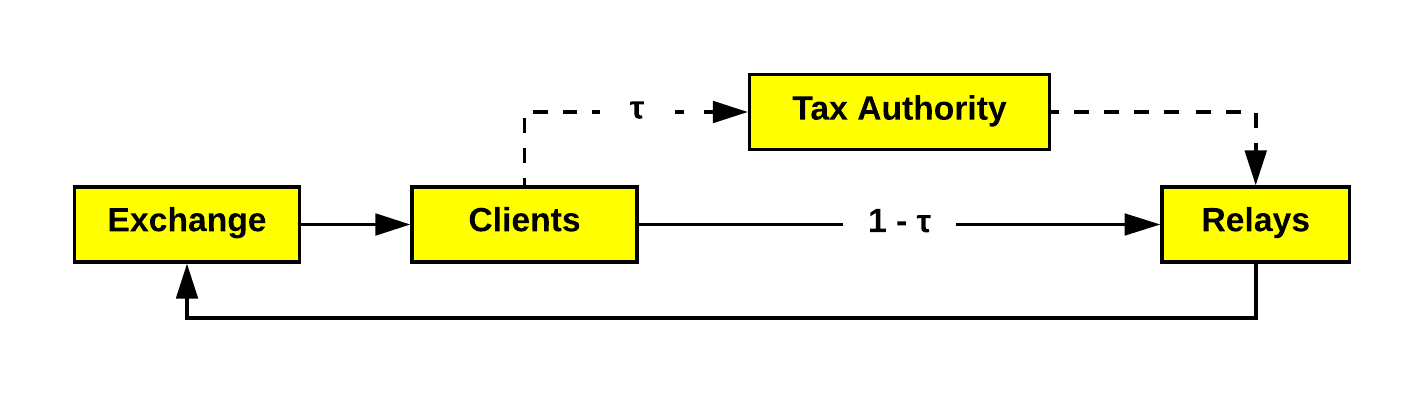
\includegraphics[trim={0.5cm, 0.5cm, 0.5cm, 0.5cm}, clip,
    scale=0.7]{images/economic_diagram.png}
  \caption[Cash Flow]{Cash Flow --- movement of moneTor tokens through the
    network. The value $\tau$ denotes the fraction of money that is collected
    for taxation purposes.}
  \label{fig:economic}
\end{figure}

We introduce a novel concept within the field in the form of a taxation element.
Intuitively, the shape of the network that will emerge in a purely
profit-seeking environment may not perfectly correspond with the central goals
of the Tor Project. The Tor Project may for instance desire to compensate
certain types of relays more than others in order to improve the overall quality
of the network (e.g., supporting areas where anonymity is particularly important
but financial resources scarce). To this end, we accommodate for a stream of
taxed income that is anonymously diverted into a shared pool of funds. These
funds are selectively redistributed to relays via a transparent policy. In
essence, taxation provides a tunable control mechanism for The Tor Project to
shape the topology of the network towards some notion of optimal diversity and
performance. The exact content of such policy is an active subject of research
that is orthogonal to our paper (e.g., Waterfilling~\cite{waterfilling-pets2017}
argues for security by maximum diversity in endpoints of user paths, and
TAPS~\cite{taps-ndss2017} argues for security by trust policies).

A key economic question to address is the issue of price determination. While it
would be tempting to enlist some market-based mechanisms to set premium
bandwidth prices, any price differentiation between clients or relays inevitably
leaks more information. This leakage becomes more severe with higher granularity
payment options as adversaries begin to use price to link payment channels and
circuits. We therefore impose the constraint that all users should pay a single
uniform price for premium bandwidth at any time $t$. This price may be set
through a centralized calculation by the authorities or a more dynamical
consensus vote reached by the network.
\subsection{Incentivized Conformity} In a decentralized network, there is no
practical way to enforce standard behavior at each local node. We must therefore
consider whether all nodes are rationally incentivized to obey the stipulated
policies. For instance, we cannot guarantee that relays will actually confer
premium bandwidth to paying users. Even though the relay has no particular
reason to deviate, the client should periodically monitor her bandwidth and only
make payments when they appear to be making a difference. The relationship
between the client and relay can then be modeled as a game theoretic tit-for-tat
dynamic within the immediate session. Over the long term, non-conforming relays
might be blacklisted via Tor's existing reporting system.

At the opposite end of the spectrum, relays might overly prioritize premium
circuits while rejecting all traffic from unpaid users. They might also attempt
to game the tax redistribution process to gain larger share of the proceeds. The
bandwidth measurement authorities must anticipate such modes of deviation from
the standard behavior to ensure that the risk for a relay to get blacklisted
from the network is greater than the incremental gains it might attain from
cheating. These attacks, while manageable, suggest that it would be prudent to
limit the complexity of our economic policies until we can better study
behavioral deviation dynamics in the live network.


\subsection{Monetary Policy}

Although we require that moneTor tokens have some sense of real-world value,
there are several monetary policies that The Tor Project may wish to choose
from. In a \emph{closed-loop} system, moneTor tokens would be created, managed,
and destroyed according to a public internal policy. As the tokens are fully
transferable, we would expect that side-markets would emerge in which they could
be traded for external assets. This system offers greater control and ability
for The Tor Project to react to economic fluctuations. However, it requires a
categorically new level of trust on the part of authorities to responsibly
manage money and monetary policy. Alternatively, in an \emph{open-loop} system,
moneTor tokens would act as a wrapper for some existing external cryptocurrency.
In this scenario, Tor would operate its own ledger and make use of one of
several protocols that have emerged in the cyptocurrency space allowing the
secure inter-ledger exchange of financial assets~\cite{back2014enabling,
  poon2017plasma}. The \emph{open-loop} approach eliminates many trust
assumptions that would otherwise be required of The Tor Project while deferring
economic responsibility away from the decision makers. However, it necessarily
couples the state of the Tor ecosystem with a likely unpredictable external
cryptocurrency. Although there are some technical considersations supporting
each option, these are likely overshadowed by political and idealogic
considerations. For the purposes of this technically-oriented paper, we will
consider this decision to be out-of-scope and design our payment protocols to
function independently of monetary policy.

% td: I think this is a little confusing without any introduction or transition
% to the next subsection

%The payment system we present in the next Section~\ref{sec:payment} is
%independent of the token creation for which multiple strategies are available.
%For example, the moneTor tokens could be viewed as wrappers for some external
%financial asset that is converted at an exchange service with an 1-to-1
%mapping. In this scenario, moneTor tokens are created when the users buy them
%with other coins and destroyed when the users sell them for other coins. A
%second example would be to let the Tor project creates and destroys moneTor
%tokens at will. In such scenario, the directory authorities handle the tokens
%as a resource management system, but do not trade them against fiat currencies
%or other coins. Given the transferability of the moneTor tokens, we would
%expect a side-market to appear for which the Tor project would not be
%responsible. These two approaches have both advantages and inconveniences
%usually linked to political opinions and ideologies.

%%% Local Variables:
%%% mode: latex
%%% TeX-master: "../main"
%%% End:
